\documentclass{article}
\usepackage{tikz}
\usetikzlibrary{patterns,shadings}
\begin{document}
% 路径类型
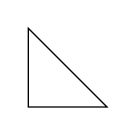
\begin{tikzpicture}
    % 1.描边线
    %   \path[draw],可简写为\draw
    \path[draw] (0,0) -- (1,0) -- (0,1) -- cycle;
\end{tikzpicture}\vspace{1cm}



\begin{tikzpicture}
    % 2.内容填充
    %   \path[fill],可简写为\fill
    %   必须为闭合线条
    \path[fill] (0,0) -- (1,0) -- (0,1) -- cycle;
\end{tikzpicture}\vspace{1cm}

% 同一命令,图形重叠部分的填充方式
% 1.nonzero rule
%   判断point是否在多层path内部,将point作为一个光源,并设置一个初始为0的数num
%   当发射的光碰到一层path时,如果路径方向(光的视角)为从左到右,则num加1;如果路径为从右到左,则num减1
%   在光到达path外部时,如果num不为0,则认为point在path内部(填充);为0,则在外部(不填充)
% 默认方式
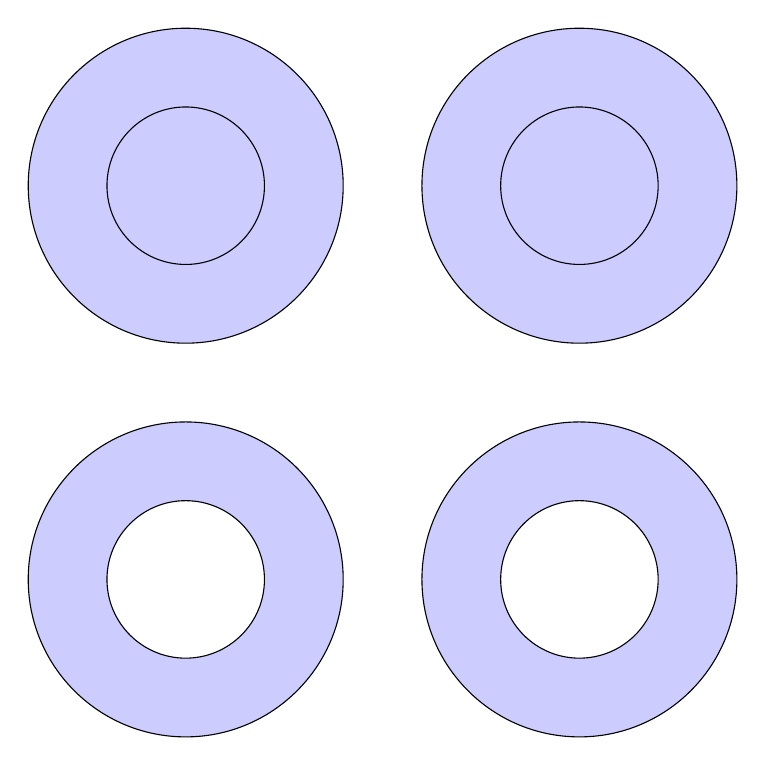
\begin{tikzpicture}
    \filldraw[fill=blue!20] (2,0) arc [start angle=0,end angle=360,radius=2] (1,0) arc [start angle=0,end angle=360,radius=1];
    \filldraw[fill=blue!20] (7,0) arc [start angle=360,end angle=0,radius=2] (6,0) arc [start angle=360,end angle=0,radius=1];
    \filldraw[fill=blue!20] (2,-5) arc [start angle=0,end angle=360,radius=2] (1,-5) arc [start angle=360,end angle=0,radius=1];
    \filldraw[fill=blue!20] (7,-5) arc [start angle=360,end angle=0,radius=2] (6,-5) arc [start angle=0,end angle=360,radius=1];
\end{tikzpicture}

% 2.even odd rule,图形相交部分直接留白
%   判断point是否在多层path内部,将point作为一个光源,并设置一个初始为0的数num
%   当发射的光碰到一层path时,如果路径方向(光的视角)为从左到右,则num加1;如果路径为从右到左,则num减1
%   在光到达path外部时,如果num为奇数,则认为point在path内部(填充);为偶数,则在外部(不填充)
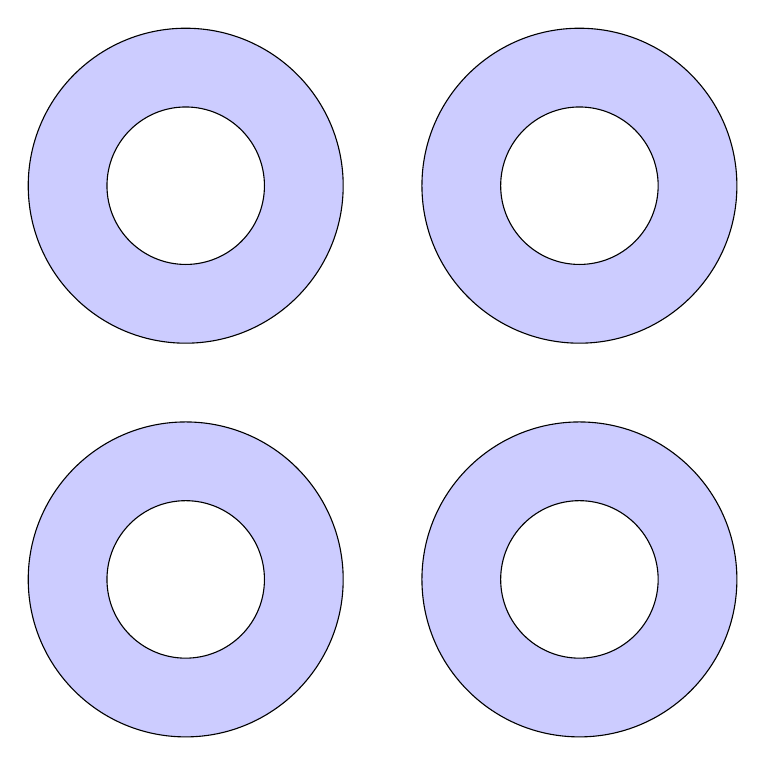
\begin{tikzpicture}
    \filldraw[fill=blue!20,even odd rule] (2,0) arc [start angle=0,end angle=360,radius=2] (1,0) arc [start angle=0,end angle=360,radius=1];
    \filldraw[fill=blue!20,even odd rule] (7,0) arc [start angle=360,end angle=0,radius=2] (6,0) arc [start angle=360,end angle=0,radius=1];
    \filldraw[fill=blue!20,even odd rule] (2,-5) arc [start angle=0,end angle=360,radius=2] (1,-5) arc [start angle=360,end angle=0,radius=1];
    \filldraw[fill=blue!20,even odd rule] (7,-5) arc [start angle=360,end angle=0,radius=2] (6,-5) arc [start angle=0,end angle=360,radius=1];
\end{tikzpicture}\newpage


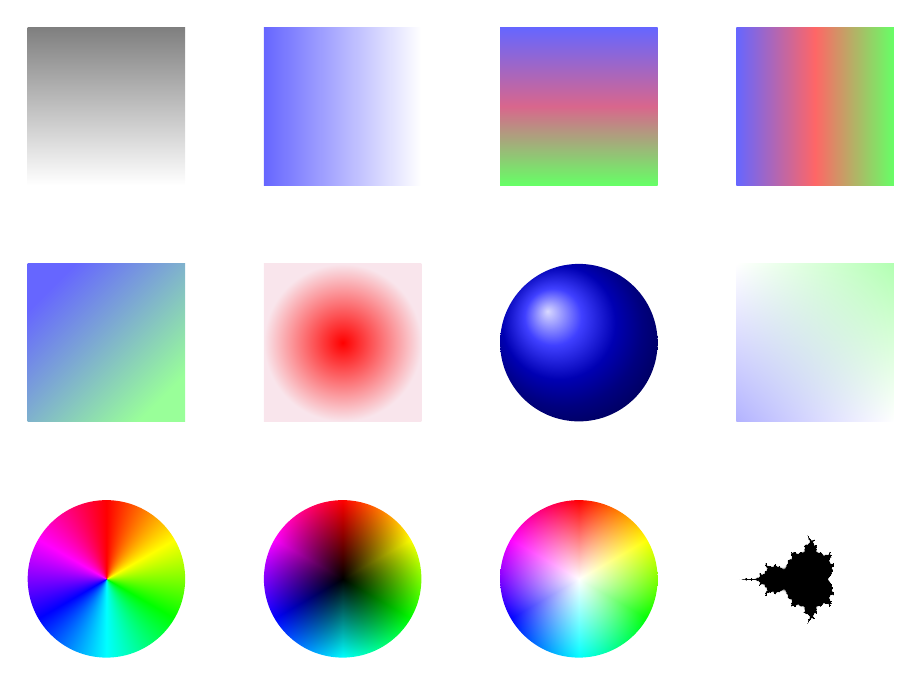
\begin{tikzpicture}
    % 3.填充内容从一个颜色平滑过渡到另一个颜色
    %   \path[shade],可简写为\shade,需使用shadings库. 参考15.7和 section 69
    %   1)axis模式, 左右或上下的线性颜色变化. 默认模式
    %     使用shading=axis指定模式,默认为从上到下,由灰色过渡到白色
    %     可使用如下参数: top color/bottom color/left color/right color/middle color
    %     middle color可结合top color/bottom color, 成为垂直中间颜色; middle color也可结合left color/right color, 成为水平中间颜色. middle color必须在top/bottom/left/right color之后使用
    %     shading angle可用于基于top/bottom旋转渐变方向,left/right默认为90
    \shade (0,0) rectangle (2,2);
    \shade[xshift=3cm,left color=blue!60] (0,0) rectangle (2,2);
    \shade[xshift=6cm,top color=blue!60,bottom color=green!60,middle color=purple!60] (0,0) rectangle (2,2);
    \shade[xshift=9cm,left color=blue!60,right color=green!60,middle color=red!60] (0,0) rectangle (2,2);
    \shade[yshift=-3cm,left color=blue!60,right color=green!40,shading angle=45] (0,0) rectangle (2,2);

    %   2)radial模式,由一点以半径向外扩散转化颜色
    %     使用shading=radial指定模式
    %     使用inner color指定中心颜色,outer color指定边缘颜色. 默认圆心为灰色,边缘颜色为白色
    \shade[shift={(3,-3)},shading=radial,inner color=red,outer color=purple!10] (0,0) rectangle (2,2);

    %   3)ball模式, 球体光影变化
    %     使用shading=ball指定模式,默认为蓝色
    %     可使用ball color指定颜色
    \shade[shift={(6,-3)},shading=ball] (1,1) circle [radius=1cm];

    %   4)bilinear interpolation模式,双线性
    %     使用shading=bilinear interpolation指定模式,需要导入shadings tikz库
    %     可使用以下关键字指定左上/右上/左下/右下颜色: upper left/upper right/lower left/lower right,默认都为白色
    \shade[shift={(9,-3)},shading=bilinear interpolation,upper right=green!30,lower left=blue!30] (0,0) rectangle (2,2);

    %   5)color wheel模式,车轮式颜色轮替
    %     使用shading=color wheel指定模式,需要导入shadings tikz库
    \shade[yshift=-6cm,shading=color wheel] (1,1) circle [radius=1cm];

    %   6)color wheel black center模式,车轮式颜色轮替,中心为黑色
    %     使用shading=color wheel black center指定模式,需要导入shadings tikz库
    \shade[shift={(3,-6)},shading=color wheel black center] (1,1) circle [radius=1cm];
    
    %   7)color wheel white center模式,车轮式颜色轮替,中心为白色
    %     使用shading=color wheel white center指定模式,需要导入shadings tikz库
    \shade[shift={(6,-6)},shading=color wheel white center] (1,1) circle [radius=1cm];

    %   8)Mandelbrot set模式,趣味性形状
    %     使用shading=Mandelbrot set指定模式,需要导入shadings tikz库
    \shade[shift={(9,-6)},shading=Mandelbrot set] (0,0) rectangle (2,2);
\end{tikzpicture}\newpage

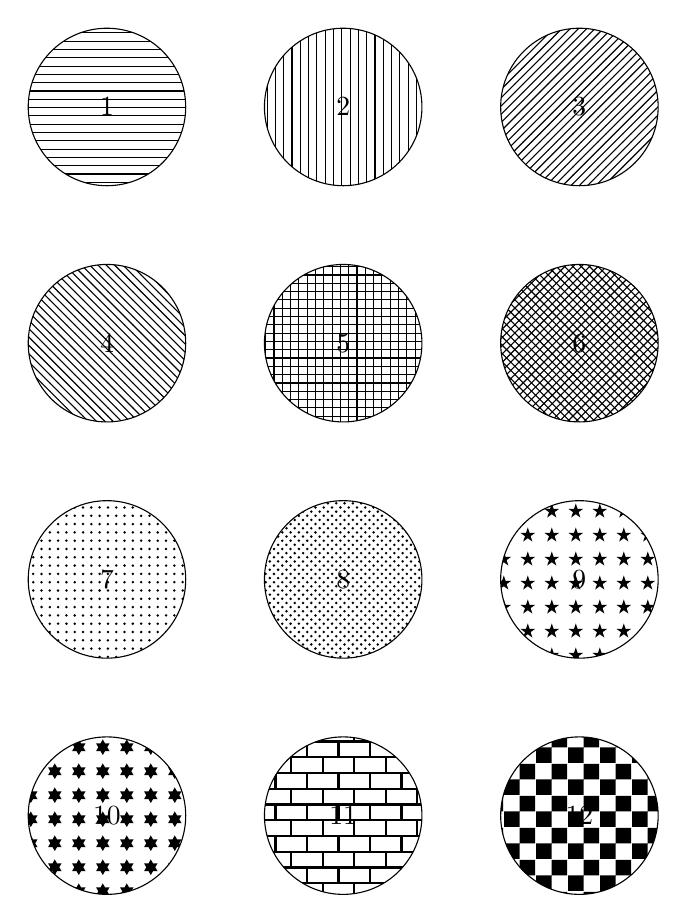
\begin{tikzpicture}
    % 4.使用预定义图形进行填充, 需要使用patterns库
    %   \path[pattern]指定填充, 可简写为\pattern(section 62). 相关参数
    %     pattern - 指定填充图形
    %     pattern color - 指定填充图形的颜色
    \draw[pattern=horizontal lines] (0,0) circle [radius=1cm];
    \node at (0,0){1};
    \draw[pattern=vertical lines,xshift=3cm] (0,0) circle [radius=1cm];
    \node[xshift=3cm] at (0,0){2};
    \draw[pattern=north east lines,xshift=6cm] (0,0) circle [radius=1cm];
    \node[xshift=6cm] at (0,0){3};
    \draw[pattern=north west lines,yshift=-3cm] (0,0) circle [radius=1cm];
    \node[yshift=-3cm] at (0,0){4};
    \draw[pattern=grid,shift={(3cm,-3cm)}] (0,0) circle [radius=1cm];
    \node[shift={(3cm,-3cm)}] at (0,0){5};
    \draw[pattern=crosshatch,shift={(6cm,-3cm)}] (0,0) circle [radius=1cm];
    \node[shift={(6cm,-3cm)}] at (0,0){6};
    \draw[pattern=dots,yshift=-6cm] (0,0) circle [radius=1cm];
    \node[yshift=-6cm] at (0,0){7};
    \draw[pattern=crosshatch dots,shift={(3cm,-6cm)}] (0,0) circle [radius=1cm];
    \node[shift={(3cm,-6cm)}] at (0,0){8};
    \draw[pattern=fivepointed stars,shift={(6cm,-6cm)}] (0,0) circle [radius=1cm];
    \node[shift={(6cm,-6cm)}] at (0,0){9};
    \draw[pattern=sixpointed stars,yshift=-9cm] (0,0) circle [radius=1cm];
    \node[yshift=-9cm] at (0,0){10};
    \draw[pattern=bricks,shift={(3cm,-9cm)}] (0,0) circle [radius=1cm];
    \node[shift={(3cm,-9cm)}] at (0,0){11};
    \draw[pattern=checkerboard,shift={(6cm,-9cm)}] (0,0) circle [radius=1cm];
    \node[shift={(6cm,-9cm)}] at (0,0){12};
\end{tikzpicture}\newpage


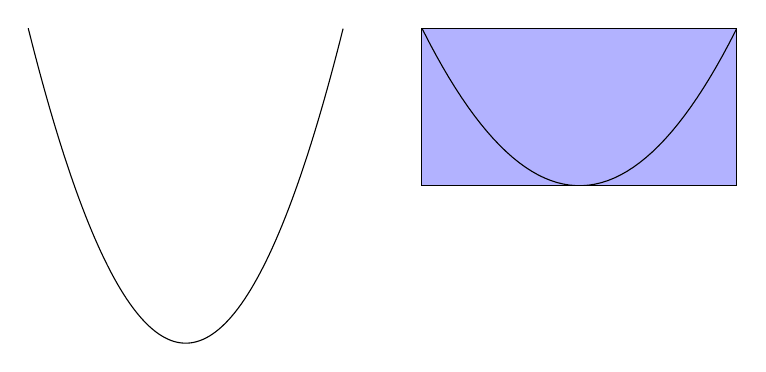
\begin{tikzpicture}
    % 5.对之后的内容,作区域保留;之前的内容,不作区域限制
    %   \path[clip],可简写为\clip
    \begin{scope}[shift={(5cm,2cm)},scale=2,fill=blue!30]
        \path[fill,draw,clip] (-1,0) rectangle (1,1);
        \path[draw] plot[samples=100,domain=-2:2] (\x,\x*\x);
    \end{scope}
    \path[name=para,draw] plot[samples=100,domain=-2:2] (\x,\x*\x);
\end{tikzpicture}\newpage


% 6.连线类型-I:
%   1)move to - 代表两点之间不连接,直接由上一个点,跳到下一个点
%   2)line to - 代表两点之间使用直线连接. 通常结尾使用cycle,使线条闭合
%   3)(p) |- (q)
%     分别取坐标p的x值,坐标q的y值,组成(x,y),并依次连接(p) -- (x,y) -- (q)
%     (p) -| (q)
%     分别取坐标p的y值,坐标q的x值,组成(x,y),并依次连接(p) -- (x,y) -- (q)
\begin{tikzpicture}
    \draw (0,0) -- (1,0) (2,0) -- (3,0);

    \begin{scope}[line width=2pt,yshift=-2cm]
        \draw (0,0) -- (1,0) -- (0,1) -- cycle;
        \draw[xshift=4cm] (0,0) -- (1,0) -- (0,1) -- (0,0);
    \end{scope}

    \begin{scope}[yshift=-4cm]
        \draw[->] (-1.5,0) -- (1.5,0) node[below]{$x$};
        \draw[->] (0,-1.5) -- (0,1.5) node[left]{$y$};
        \draw[red] (0,0) -| (1,1);
    \end{scope}
\end{tikzpicture}\vspace{1cm}

% 6.连线类型-II:
%   4)曲线,使用(<first_point>) .. controls (<first_control_point>) and (<second_control_point>) .. (<second_point>)
%     原理: 第一个点first_point的切线指向第一个控制点first_control_point,第二个点second_point的切线指向第二个控制点second_control_point
%     如果省略 and (<second_control_point>),则第二个点second_point的切线也指向第一个控制点first_control_point
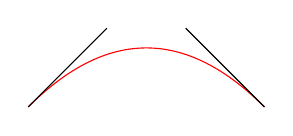
\begin{tikzpicture}
    \draw[red] (0,0) .. controls (1,1) and (2,1) .. (3,0);
    \draw (0,0) -- (1,1) (2,1) -- (3,0);
\end{tikzpicture}





% 常用图形形状
\begin{tikzpicture}
    % 圆
    %   (<central>) circle [radius=<radius>]
    \draw (0,0) circle [radius=1];

    % 椭圆
    %   (<central>) circle [x radius=<x_radius>,y radius=<y_radius>]
    \draw (3,0) ellipse [x radius=1,y radius=0.5];

    % 长方形
    %   (<coordinate>) rectangle (<diagonal_coordinate>)
    \draw (5,-1) rectangle (7,1);

    % 圆弧
    %   (<start_point_coordinate>) arc [start angle=<start_angle>,end angle=<end_angle>,radius=<radius>]
    \draw (1,-3) arc [start angle=0,end angle=180,radius=1];
    
    % 椭圆弧
    %   (<start_point_coordinate>) arc [start angle=<start_angle>,end angle=<end_angle>,x radius=<x_radius>,y radius=<y_radius>]
    \draw (2,-3) arc [start angle=180,end angle=360,x radius=1,y radius=0.5];
\end{tikzpicture}
    
    

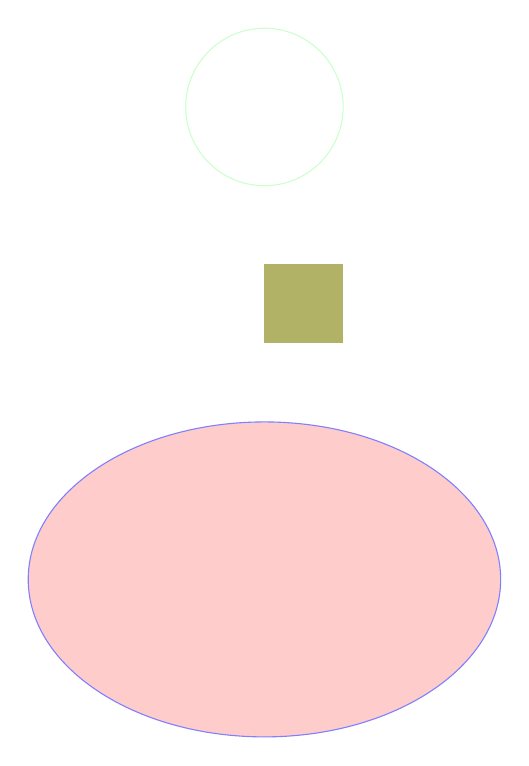
\begin{tikzpicture}
    % 填充颜色: 自定义颜色和颜色表达式,可使用latex的xcolor宏包
    % draw中, color指定边框颜色
    \draw[color=green!20] (0,3) circle [radius=1cm];
    % fill中, color指定填充颜色
    \fill[color=red!50!green!60] (0,0) rectangle (1,1);
    % filldraw中,color指定填充和边框颜色,fill指定填充颜色,draw指定边框颜色
    \filldraw[color=blue!50,fill=red!20] (0,-3) ellipse [x radius=3cm,y radius=2cm];
\end{tikzpicture}\vspace{1cm}


\begin{tikzpicture}
    % 坐标顶点是圆角/尖角
    % rounded corners=<dimension>
    %   圆滑的边角弧度,dimension值不被scale影响
    % sharp corners
    %   尖锐的边角弧度
    % 可以在路径中使用,影响后续顶点弧度
    \draw (0,0) -- (2,0) -- (2,1) -- (0,1) -- cycle;
    \draw[xshift=4cm,rounded corners=5pt] (0,0) -- (2,0) -- (2,1) -- (0,1) -- cycle;
    \draw[yshift=-2cm] (0,0) -- (2,0) -- (2,1) [rounded corners=5pt] -- (0,1) -- cycle;
\end{tikzpicture}


% update 2025-04-15





\begin{tikzpicture}
    % 1.指定线条粗细: 
    %   line width=<dimension>
    % 使用预定义宽度: 
    %   1)ultra thin
    \draw[ultra thin] (-2,1) -- (2,1);
    %   2)very thin
    \draw[very thin] (-2,0.5) -- (2,0.5);
    %   3)thin(默认,即0.4pt)
    \draw[thin] (-2,0) -- (2,0);
    \draw (-2,-0.5) -- (2,-0.5);
    %   4)semithick
    \draw[semithick] (-2,-1) -- (2,-1);
    %   5)thick
    \draw[thick] (-2,-1.5) -- (2,-1.5);
    %   6)very thick
    \draw[very thick] (-2,-2) -- (2,-2);
    %   7)ultra thick
    \draw[ultra thick] (-2,-2.5) -- (2,-2.5);
\end{tikzpicture}\newpage

\begin{tikzpicture}
    % 线条类型: tikz的线条主要由虚线来实现
    % 1.dash pattern=on 2pt off 3pt on 4pt off 4pt
    %   代表画2pt线条,间隔3pt,再画4pt线条,再间隔4pt
    % 2.dash phase=3pt
    %   将通过dash pattern配置的虚线,左移3pt
    % 3.dash=<pattern> phase <phase>
    %   合并1/2步
    % 4.其他预定义线条
    %   1)solid - 实线. 默认类型
    %   2)dotted/densely dotted/loosely dotted - 点线/密集点线/稀疏点线
    %   3)dashed/densely dashed/loosely dashed - 虚线/密集虚线/稀疏虚线
    %   4)dash dot/densely dash dot/loosely dash dot - 虚点线/密集虚点线/稀疏虚点线
    %   5)dash dot dot/densely dash dot dot/loosely dash dot dot - 虚点点线/密集虚点点线/稀疏虚点点线
    \draw[loosely dashed] (-2,0) -- (2,0);
    \draw[dashed] (-2,-0.5) -- (2,-0.5);
    \draw[densely dashed] (-2,-1) -- (2,-1);
    \draw (-2,-1.5) -- (2,-1.5);
    \draw[solid] (-2,-2) -- (2,-2);
    \draw[loosely dotted] (-2,-2.5) -- (2,-2.5);
    \draw[dotted] (-2,-3) -- (2,-3);
    \draw[densely dotted] (-2,-3.5) -- (2,-3.5);
\end{tikzpicture}





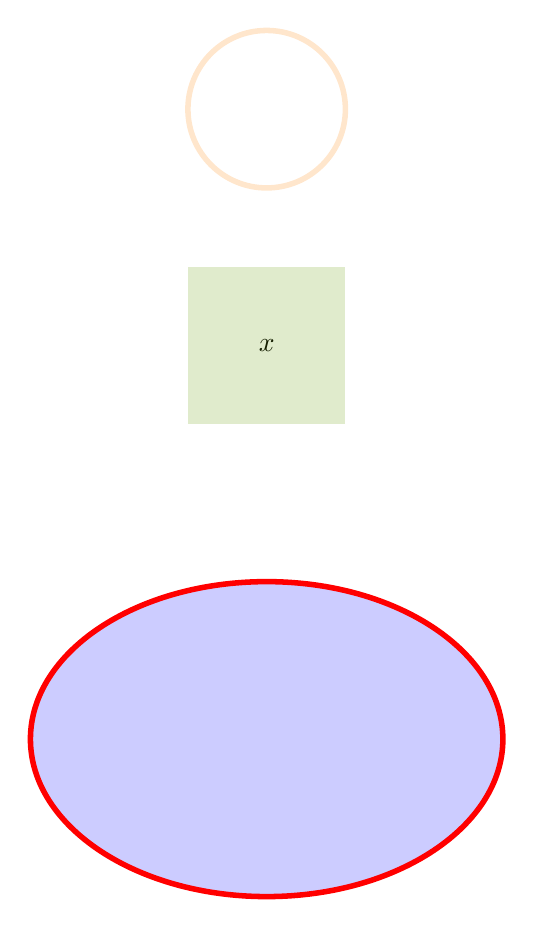
\begin{tikzpicture}
    % 透明度,范围[0,1],0代表完全透明,1代表完全不透明
    \node at (0,0) {$x$};
    % draw中,opacity指定边框透明度
    \draw[color=orange,line width=2pt,opacity=0.2] (0,3) circle [radius=1cm];
    % fill中,opacity指定填充透明度
    \fill[color=red!40!green,opacity=0.2] (-1,-1) rectangle (1,1);
    % filldraw中,fill opacity指定填充透明度,draw opacity指定边框透明度,opacity指定填充和边框透明度
    \filldraw[line width=2pt,draw=red,fill=blue,fill opacity=0.2] (0,-5) ellipse [x radius=3cm,y radius=2cm];
\end{tikzpicture}\newpage

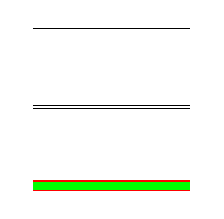
\begin{tikzpicture}
    % 单线与双线
    % 可使用double参数的属性值指定线条间填充颜色
    % double distance指定线条间的距离
    \draw (0,1) -- (2,1);
    \draw[double] (0,0) -- (2,0);
    \draw[double,red,double=green,double distance=3pt] (0,-1) -- (2,-1);
\end{tikzpicture}\newpage













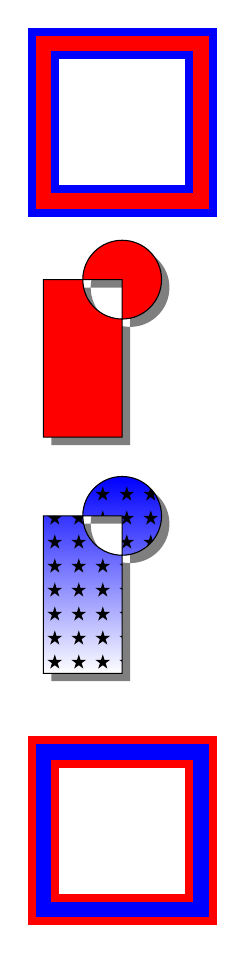
\begin{tikzpicture}
    % preaction(pre-action)参数,先进行preaction的操作,再使用指定参数作图后
    % 如图示例,先作一个宽度为2mm,颜色为蓝色的矩形;再画一个红色的矩形
    \draw 
    [preaction={draw,line width=4mm,blue}]
    [line width=2mm,red] (0,0) rectangle (2,2);
    \begin{scope}[yshift=-3cm]
	\draw 
	[preaction={fill=black,opacity=0.5,transform canvas={xshift=1mm,yshift=-1mm}}]
	[fill=red] (0,0) rectangle (1,2) circle (5mm);
    \end{scope}
    % 多次调用preaction
    \begin{scope}[yshift=-6cm]
	\draw 
	[preaction={fill=black,opacity=0.5,transform canvas={xshift=1mm,yshift=-1mm}}]
	[preaction={top color=blue,bottom color=white}]
	[pattern=fivepointed stars] (0,0) rectangle (1,2) circle (5mm);
    \end{scope}
    \begin{scope}[yshift=-9cm]
	\draw 
	[postaction={draw,line width=2mm,blue}]
	[line width=4mm,red] (0,0) rectangle (2,2);
    \end{scope}
\end{tikzpicture}
\end{document}
